\chapter{医学检验研究的设计}
\label{ch:13}
\chapterauthors{Thomas B. Newman、Michael A. Kohn、Warren S. Browner、Mark J. Pletcher}
\newcommand{\chthirteenroc}{%
\begin{tikzpicture}[x=.23mm,y=.23mm]
\node[anchor=south west,inner sep=0] at (0,0)
 {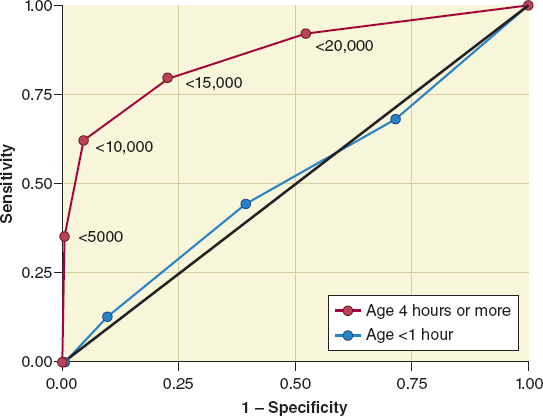
\includegraphics[width=124.89mm]{assets/ch13_roc_original.png}};
% Cover only the English axis titles and legend text; keep all data marks and ticks.
\fill[white] (0,130) rectangle (18,280);
\node[rotate=90,font=\small] at (8,207) {灵敏度};
\fill[white] (215,0) rectangle (355,22);
\node[font=\small] at (290,10) {$1-$特异度};
\fill[white] (364,69) rectangle (516,119);
\node[anchor=west,font=\small] at (366,105) {出生 $\geq4$ 小时};
\node[anchor=west,font=\small] at (366,80) {出生 $<1$ 小时};
\end{tikzpicture}}
\newcommand{\chthirteentree}{%
\begin{tikzpicture}[x=1mm,y=1mm,>=Latex,
 decision/.style={draw=dcrblue!70,fill=dcrlight,rounded corners=2pt,
 align=center,text width=39mm,font=\small,inner sep=3mm},
 high/.style={draw=red!65!black,fill=red!65!black,text=white,rounded corners=2pt,
 align=center,text width=34mm,font=\small,inner sep=3mm},
 low/.style={draw=green!45!black,fill=green!15!gray!25,rounded corners=2pt,
 align=center,text width=34mm,font=\small,inner sep=3mm}]
\node[decision,text width=63mm] (root) at (0,0)
 {908 名 $<60$ 日龄婴儿，\\82 名（9\%）有严重细菌感染};
\node[decision] (ua) at (0,-25) {尿液分析阳性？};
\node[high] (h1) at (-30,-52) {较高风险\\$63/127=50\%$};
\node[decision] (anc) at (25,-52) {中性粒细胞绝对计数\\$>4090/\mu$L？};
\node[high] (h2) at (0,-82) {较高风险\\$15/248=6\%$};
\node[decision] (pct) at (55,-82) {降钙素原\\$>1.71$ ng/mL？};
\node[high] (h3) at (25,-113) {较高风险\\$3/11=27\%$};
\node[low] (l) at (85,-113) {低风险\\$1/522=0.2\%$};
\draw[->,thick] (root)--(ua);
\draw[->,thick] (ua)--(h1);
\draw[->,thick] (ua)--(anc);
\draw[->,thick] (anc)--(h2);
\draw[->,thick] (anc)--(pct);
\draw[->,thick] (pct)--(h3);
\draw[->,thick] (pct)--(l);
\end{tikzpicture}}

\sourcepage{412}
医学检验研究是临床研究的重要组成部分，检验可用于筛查危险因素、诊断疾病或估计患者预后。这里所说的检验，也包括由多项原始测量组成的风险评分。本章讨论的研究设计，可以用于研究某种检验是否应当开展，以及应当用于哪些人。

多数医学检验研究的设计，与第 8、9 章的观察性设计相似，但有几项重要差别。最重要的是，多数观察性研究旨在发现代表因果效应的统计学显著关联。相反，证明检验结果与某种疾病存在统计学显著关联，并不能确定该检验是否具有临床用途；而且对多数医学检验研究而言，因果关系并不相关。因此，关联指标、统计学显著性和混杂控制是次要考虑。这类研究主要关注灵敏度、特异度、受试者工作特征曲线（receiver operating characteristic curves，ROC 曲线）、似然比（likelihood ratios，LR），以及相应置信区间（CI）等描述性参数。最后，医学检验研究几乎总是在患者中开展，因此本章均使用“患者”一词。

\section{确定检验是否有用}
一项检验要有用，必须经受一系列越来越难的问题，涉及可重复性、准确度、可行性，以及最重要的——它对临床决策与结局的影响（表 13.1）。只有所有问题都得到肯定回答，\sourcepage{413}才有把握认为值得开展这项检验。毕竟，如果检验因操作者或场所不同而产生很不相同的结果，就不大可能有用。如果它很少提供新信息，就不大可能影响临床决策。即使能影响决策，如果这些决策不能在合理风险和成本下，改善受检患者的临床结局，它仍可能没有用。

\begingroup\small
\begin{longtable}{L{30mm}L{58mm}L{57mm}}
\caption*{\textbf{表 13.1\quad 判断医学检验用途的问题、可用的研究设计及结果报告指标}}\\
\toprule\textbf{问题}&\textbf{可能的设计}&\textbf{报告结果的统计量$^{a}$}\\\midrule\endfirsthead
\toprule\textbf{问题}&\textbf{可能的设计}&\textbf{报告结果的统计量$^{a}$}\\\midrule\endhead
检验的可重复性如何？&研究观察者内、观察者间，以及实验室内、实验室间变异。&一致比例、kappa、变异系数、差值均值及分布、Bland–Altman 图（避免使用相关系数）。\\
检验诊断疾病的准确度如何？&横断面、病例对照或按检验结果抽样的设计，将检验结果与金标准比较。&灵敏度、特异度、阳性与阴性预测值、ROC 曲线、似然比。\\
检验或预测模型预测结局的准确度如何？&以检验结果估计发生结局概率的队列设计。&风险比、风险率比、绝对风险、ROC 曲线、校准图、净获益计算。\\
检验是否可行、能否负担？&前瞻性或回顾性研究，与现行标准诊疗比较。&平均成本、发生不良反应的比例、愿意接受检验的比例。\\
\sourcepage{414}
检验结果多常影响临床决策？&诊断检出率研究，以及检验前后临床决策研究。&异常比例、阳性者追加检查情况、导致临床决策改变的检验比例、每检出一个异常结果或每改变一次决策的成本。\\
开展检验是否改善临床结局，或产生不良影响？&随机试验、队列或病例对照研究，或决策分析、成本－效果分析；预测变量为接受检验，结局包括疾病或治疗相关的患病、死亡或成本。&风险比、比值比、风险率比、绝对风险、需治疗人数，有利与不利结局的发生率及比率，例如每避免一个不良结局所需的成本或造成的不良反应。\\\bottomrule
\multicolumn{3}{L{151mm}}{\footnotesize $^{a}$ 表中大多数统计量均应同时报告置信区间。}\\
\end{longtable}\endgroup

如果使用检验能改善受检患者的结局，就可以推断其他问题也有肯定答案。然而，研究检验能否改善患者结局，是最难开展的研究。因此，通常是通过比较新检验与现有检验的准确度、安全性或成本，推断它对结局的潜在影响。开发新的诊断或预后检验时，应考虑它要指导什么决策，现有实践中哪些方面最需改进。例如，当前检验是否不可靠、不准确、昂贵、危险，或难以实施？

\subsection{医学检验研究的一般问题}
在讨论表 13.1 中不同设计的特有问题前，先讨论医学检验研究普遍适用的几个问题。

\subsubsection{疾病严重程度谱及检验结果谱}
多数医学检验研究通过测量样本，对人群作出推断，\sourcepage{415}因此样本选择方式极大影响推断效度。当样本中的疾病谱或非疾病谱，不同于检验预定使用的临床人群时，就出现\term{疾病谱偏倚（spectrum bias）}。在开发早期，研究检验是否能区分明确的晚期患者与健康对照，可能是合理的；如果不能，研究者可以回实验室改进，或另找检验。但在后期，当问题转为临床用途时，疾病与非疾病谱，都应能代表实际将接受检验的患者。例如，一项通过比较已知胰腺癌患者与健康对照而开发的检验，随后可以在更难区分、但更贴近临床的样本中评价，如连续就诊的不明原因腹痛或体重下降者。

不恰当的检验结果谱，也会造成疾病谱偏倚。假设研究放射科医师判读乳腺 X 线摄影的一致性，让他们将影像分为正常或异常。如果研究者选出的“阳性”影像明显异常，而“阴性”影像毫无可疑异常，一致性就会高得多。

\subsubsection{盲法的重要性}
许多检验是客观的，例如自动化学分析仪检测；另一些则涉及主观判断，例如体格检查和放射影像。只要可能，研究者就应让主观检验的判读者不知受检患者的其他资料。例如，研究超声对阑尾炎诊断的贡献时，超声图像判读者不应知道病史与体格检查结果\footnote{另一种方法是比较仅用病史和体格检查的准确度，与加用超声后的准确度。}。同样，用于比较检验结果的\term{金标准}，有些客观，例如死亡；有些主观，例如病理医师判断是否有阑尾炎。金标准主观时，执行金标准者不应知道待评价检验的结果。\sourcepage{416}对检验执行者设盲，可防止偏倚、先入之见和其他来源信息影响检验结果；对金标准执行者设盲，可防止检验结果影响其判断谁有、谁没有该结局。

\par
\begin{figure}[htbp]\centering\chthirteenroc
\caption{白细胞计数（每 $\mu$L）预测新生儿感染的 ROC 曲线（10）。每个点代表判定异常的不同界值。在出生 $\geq4$ 小时时，检验表现相当好；在 $<1$ 小时时则没有价值。}\label{fig:13_01}\end{figure}\par

\subsubsection{变异来源}
对某些研究问题，患者之间的差异是检验结果变异的主要来源。例如，阑尾炎患儿中白细胞（white blood cell，WBC）计数升高的比例，预计不会因检测实验室而有很大不同。另一方面，许多结果取决于操作者或场所。例如，超声诊断阑尾炎的灵敏度、特异度及评定者间信度，取决于扫描者技能、判读者的技能与经验，以及设备质量。\sourcepage{417}如果准确度可能随判读者或机构而变化，研究不同判读者和机构，有助于评价结果是否一致。

\subsubsection{金标准并不完美}
有些疾病有普遍认可的金标准，可判断目标疾病有无，例如阑尾炎的阑尾病理检查。另一些疾病的金标准由人为规定，例如将冠状动脉造影显示一支或多支主要冠状动脉至少 50\% 狭窄，定义为冠状动脉疾病。还有些疾病，例如许多风湿性疾病，要求患者具备规定数量的体征、症状或实验室异常。当然，如果某项体征、症状或实验室检验就是金标准的一部分，它会很好地预测谁有病。这称为\term{纳入偏倚（incorporation bias）}，因为被研究的检验——常称\term{待评价检验（index test）}——被纳入了金标准。避免方法是选用不包含待评价检验的金标准；若做不到，与其研究它多大程度上预测金标准，不如研究它多大程度上预测预后或治疗反应。

还要考虑金标准是否真是“金”的。如果金标准不完美，它既可能使检验看起来比实际差（当待评价检验实际上优于金标准时（1）），也可能使它看起来比实际好（当两者犯同样的错误时（2））。

\subsubsection{过拟合的危险}
检验是在本身并不完美的研究中开发的。开发者过度解读抽样或测量误差中不可避免的随机变异与噪声，并将其纳入检验算法，就发生\term{过拟合（overfitting）}。它使检验在实际应用中的表现，差于开发研究中的表现；\sourcepage{418}这也是必须在另一人群中验证检验表现的重要原因。

例如，研究纳入 5 名卵巢癌妇女和 95 名无卵巢癌妇女，用血液检验测量血清中 500 种代谢物。仅由偶然性，许多代谢物在癌症组中就会略高；几乎肯定能找出一种非常特定的 500 种代谢物组合模式，在全部 5 名患者中出现，而所有对照都没有。但这个模式很可能不能用于筛查，因为它只是随机变异的结果。统计方法虽能评价偶然因素的作用，规范的假设检验却常跟不上检验开发中的反复调整，也无法克服多重假设检验的严重问题。

用多变量模型把多种原始测量组合为检验算法时，常出现过拟合，正如上述例子。简单检验也可能过拟合，例如给血清铁蛋白这样的连续结果选择界值。研究者可能忍不住查看全部有结局者（如缺铁性贫血）和无结局者（其他贫血）的结果，再挑一个看起来最好的阳性界值。但这也是过拟合。更好的方法是依据其他研究的临床或生物学知识确定界值，或把连续结果分成区间，为每个区间计算似然比（后文讨论）。为尽量减少过拟合，应预先规定区间界值，或采用合理的整数。独立于模型开发来评价表现的模型验证研究，将在后文临床预测模型部分讨论。

\section{检验可重复性研究}
在被测现象没有真实变化时，如果检验结果不随时间、场所或操作者改变，就具有可重复性。\term{观察者内可重复性（intraobserver reproducibility）}\sourcepage{419}描述同一观察者或实验室在不同时间对同一标本检验的结果一致程度。例如，放射科医师在两次看到同一胸片时，假定不知道自己上次的判读，能有多大比例作出相同判断？\term{观察者间可重复性（interobserver reproducibility）}描述两名或更多观察者的一致程度：另一位医师看到同一影像，有多大可能与第一位意见一致？

可重复性的高低常是主要研究问题。有时，研究它是为了改善临床诊疗或研究质量。如果观察者内或观察者间变异很大、可重复性差，测量就不大可能有用，可能需要改进或放弃。当然，所有观察者即使彼此一致，也可能全部都错。

\subsection{设计}
评价可重复性的基本设计，是比较不同观察者或不同时点取得的结果。检验若包含多个步骤，每一步的差异都可能影响可重复性，研究者必须决定研究涵盖多大范围。例如，只研究一个实验室里病理医师对一组宫颈巴氏涂片的一致性，可能高估整个巴氏涂片检验的可重复性，因为未捕捉取样和制片方法的变异。

需要在多大程度上分离导致观察者分歧的步骤，部分取决于研究目标。多数研究应估计整个检验过程的可重复性，因为它决定是否值得使用。但开发或改进检验的研究者，也许想重点研究有问题的特定步骤。不论哪种情况，都应在操作手册中详列获得结果的确切流程（第 18 章），\sourcepage{420}并在报告研究时的方法部分加以描述。

\subsection{分析}
\subsubsection{分类变量}
观察者间一致性最简单的指标，是意见完全一致的观察占比。但当各类别分布不均，例如二分类检验“异常”比例远离 50\% 时，一致百分比可能难以解释，因为它没有考虑两位观察者仅凭对异常患病率的某些了解，就可能取得一致。例如，若 95\% 的检验正常，两位观察者各随机选择 5\% 判为“异常”，他们约有 90\% 的时候都会判为“正常”。当结果多于两类且本身有序，例如正常、临界、异常时，一致百分比也不是理想指标，因为它把部分分歧（正常／临界）与完全分歧（正常／异常）同样计算。

更好的观察者间一致性指标是\term{kappa}（见附录 13A）。它衡量超过根据观察者对异常比例的估计所预期的一致程度\footnote{kappa 常被描述为“超过偶然预期的一致程度”。但对偶然一致的估计，是按每名观察者判定的异常比例计算，仿佛这个比例固定且已为他们所知；一般并非如此。}，并可对部分一致给予一定权重。kappa 范围为 $-1$（完全不一致）到 1（完全一致）。0 表示一致程度未超过根据观察者对各级异常比例的估计所预期的程度。通常认为大于 0.8 非常好，0.6—0.8 较好。

\subsubsection{连续变量}
研究两台仪器或两种方法的一致性时，例如对一组患者用不同体温计取得配对体温，可先计算同一个人近乎同时的两次测量差值，\sourcepage{421}直接描述这些差值，例如计算均值及标准差。也可以将差值对两次测量的均值作图，即 Bland–Altman 图，以了解不同测量范围的可重复性是否不同（3）。另一方法是报告两次测量差值超过某个临床重要界限的频率。例如，若 0.3\,°C 是体温的临床重要差异，一项比较非接触红外体温计与电子腋温计的研究，可以估计两种方法差值的均值与标准差，并报告差值 $>0.3$\,°C 的频率\footnote{虽然常用，实验室检验信度研究最好避免使用相关系数，因为它很受离群值影响，也不能让读者判断两次测量的差异多常具有临床重要性。同样应避免仅报告平均差值的置信区间，因为它取决于样本量，可能误导。平均差值的区间很窄，并不意味着每对测量通常很接近，只表示平均差值估计得很精确。详见 Bland 与 Altman（3），或 Newman 与 Kohn（4）。}。

测量值越大，变异也常越大。例如，血压约为 120/80 mmHg 时可波动 $\pm4$ mmHg，180/120 mmHg 时可波动 $\pm6$ mmHg；Bland–Altman 图能清楚显示这一关系。这时可以用\term{变异系数（coefficient of variation，CV）}概括，即同一标本全部测量结果的标准差除以均值（第 4 章）。该指标常用于比较大量不同技术人员、实验室或仪器的批次间、观察者间或仪器间变异。也常比较两种或更多检测方法或仪器的 CV；CV 最小者精密度最高，但准确度未必最高。

\section{检验准确度研究}
本节研究回答“检验多常给出正确答案”。当然，这假定存在一个能揭示正确答案的金标准。

\subsection{设计}
准确度研究的设计，取决于检验是用于诊断现存疾病的\term{诊断性检验（diagnostic test）}，还是用于预测尚未发生结局的\term{预后性检验（prognostic test）}\footnote{另一种常见区分是诊断性检验与筛查检验；后者用于没有已知相关体征或症状的人。为简化讨论，本章“诊断性检验”一般也包括筛查检验。}。\sourcepage{422}诊断性检验研究采用横断面时间框架，测量其识别独立金标准所确定目标疾病的能力。预后性检验研究采用纵向时间框架，既测量区分发生与不发生结局者的能力（区分度），也测量预测患者组风险的准确程度（校准度）。

\subsubsection{抽样}
\textbf{多数诊断准确度研究采用类似病例对照或横断面研究的设计。}病例对照设计分别抽取有病和无病者，再比较两组检验结果。

如前所述，开发早期若要判断检验是否值得继续研究，尤其疾病罕见时，病例对照抽样可能适合。后期研究临床用途时，疾病谱和非疾病谱应类似实际应用人群，即诊断尚未知者。病例对照抽样较难做到，因为病例已经确诊，而曾考虑该诊断、后来又排除的对照也可能难找。此外，执行和／或判读检验者可能已知诊断，导致测量或报告偏倚，这也是设盲的理由。

第 3 章指出，连续抽样是取得代表性样本的好方法。连续纳入为某一诊断接受评估的患者，通常可获得具有代表性的疾病谱和非疾病谱。例如，Tokuda 等（5）发现，寒战程度——如感到冷，或盖厚被仍全身发抖——能有力预测急诊发热成人的菌血症。患者在菌血症状态尚未知时就已纳入，\sourcepage{423}因此应能较好代表类似的急诊发热患者。

后文“差异核实偏倚”将讨论，对待评价检验阴性者实施有创金标准，可能不符合伦理或不可行。即使金标准无创，若阴性结果很多，对每个人都做也可能效率低。这时可仿照第 8 章双队列设计，分别抽取阳性和阴性者，即\term{按检验结果抽样（test-result-based sampling）}。例如，对全部阳性者实施金标准，只对随机抽取的部分阴性者实施金标准，再用简单代数估计灵敏度、特异度和似然比。

比较两种可能均不完美的检验时，有时采用较高效的\term{并行配对检验（tandem testing）}：在具有代表性的患者样本中，两项检验都做；对一项或两项阳性者，有选择地实施金标准。还应对两项均阴性者随机抽取一部分实施金标准，确认确实无病。这使研究者不必支付为全部阴性者实施金标准的费用，也能判断哪项检验更准确。比较不同宫颈细胞学方法的研究，曾采用这一设计（6）。

预后检验准确度研究需要队列设计。前瞻性设计在起点时检验，再随访谁发生结局。若新检验问世，而已有保存血样的既定队列，就可采用回顾性队列或巢式病例对照设计。例如，血清神经丝轻链（serum neurofilament light chain，sNfL）可作为多发性硬化的早期征象（7），可测定储存血样的 sNfL，判断能否预测发病。结局罕见、检验昂贵时，巢式病例对照设计尤其有吸引力（第 9 章）。

\sourcepage{424}
\subsubsection{预测变量：检验结果}
把结果看成阳性或阴性最简单，但许多检验产生分类、有序或连续结果。为充分利用全部信息，通常应报告有序或连续结果，而非简单二分成“正常／异常”。多数检验在高度异常时，比轻度异常更提示疾病；临界范围则通常不能提供多少信息。

\subsubsection{结局变量：疾病或其结局}
诊断检验研究的结局变量是疾病有无，最好用金标准确定。\textbf{只要可能，结局评价就不应受待研究诊断检验结果的影响。}最好的办法是对金标准判定者设盲，使其不知待研究检验的结果。

有时，特别是筛查检验，统一实施金标准不符合伦理或不可行。例如，Smith-Bindman 等（8）研究乳腺 X 线摄影准确度。阳性妇女被转诊进一步检查，最终以活检病理为金标准，区分真阳性和假阳性。但对阴性妇女做乳腺活检并不合理。为判断她们是假阴性还是真阴性，作者把摄影结果与当地肿瘤登记相连接，查看随后一年是否诊断乳腺癌。这假定摄影时已经存在的所有乳腺癌都会在一年内确诊，也假定一年内确诊的癌在摄影时都已存在。根据检验结果采用不同金标准，可能产生偏倚，章末将详述；但有时这是唯一可行的办法。

\sourcepage{425}
预后检验研究的结局变量涉及患者以后怎样，例如存活多久、出现什么并发症、需要什么额外治疗。盲法仍然重要，尤其是临床医师可能根据被研究的预后因素作决定时。

一个问题是，较差的预后可能成为自我实现的预言，使预后检验显得比本来的预测能力更强。例如，Rocker 等（9）发现，主治医师对预后的估计与重症监护病房死亡有关，床旁护士的估计则没有。可能是主治医师更善于判断病情严重程度，也可能是他们的估计比护士更影响撤除生命支持的决定。要区分两者，可请未参与作出或引导撤除支持决定的其他主治医师估计预后。

相反，如果令人担忧的结果引发治疗并改善预后，检验或评分的预测能力反而会下降。例如，患者能获得高效抗逆转录病毒治疗时，HIV 阳性预测 10 年死亡的能力会大为减弱。

\subsection{分析}
\subsubsection{灵敏度、特异度、阳性与阴性预测值及准确率}
二分类检验与二分类金标准的比较，可用 $2\times2$ 表概括（表 13.2）。\term{灵敏度（sensitivity）}是有病患者中，检验回答正确、即阳性的比例；\term{特异度（specificity）}是无病患者中，检验回答正确、即阴性的比例。如果样本代表预定使用人群，还可计算两个参数：\term{阳性预测值（positive predictive value）}是阳性者中有病的比例，\sourcepage{426}\term{阴性预测值（negative predictive value）}是阴性者中无病的比例。

\begin{center}\small
\captionof*{table}{\textbf{表 13.2\quad 用 $2\times2$ 表概括二分类检验研究结果}}
\begin{tabularx}{\linewidth}{L{19mm}L{25mm}L{25mm}L{23mm}Y}
\toprule&\multicolumn{2}{c}{\textbf{金标准}}&&\\
\textbf{检验}&\textbf{有病}&\textbf{无病}&\textbf{合计}&\\\midrule
阳性&$a$，真阳性&$b$，假阳性&$a+b$&阳性预测值$^{*}=a/(a+b)$\\
阴性&$c$，假阴性&$d$，真阴性&$c+d$&阴性预测值$^{*}=d/(c+d)$\\
合计&$a+c$&$b+d$&$a+b+c+d$&\\\midrule
&灵敏度 $=a/(a+c)$&特异度 $=d/(b+d)$&\multicolumn{2}{l}{准确率 $=\dfrac{a+d}{a+b+c+d}$}\\\bottomrule
\end{tabularx}
\par\smallskip\begin{minipage}{\linewidth}\footnotesize
$^{*}$只有疾病患病率为 $(a+c)/(a+b+c+d)$ 时，才能由这样的表计算阳性和阴性预测值。若有病与无病者分别抽样，例如病例对照抽样各取 100 人，便不符合这一条件。
\end{minipage}\end{center}

另一项有时用于诊断检验的指标是\term{准确率（accuracy）}，即全部患者中检验回答正确的比例。它是按样本患病比例加权的灵敏度与特异度平均值。因此它不是很有帮助的统计量：对于患病率 $<1\%$ 的疾病，一项始终报阴性的无用检验，也可有 $>99\%$ 的准确率。

\subsubsection{受试者工作特征曲线}
许多诊断检验产生有序或连续结果。随着阳性界值改变，灵敏度和特异度会有多种可能组合。\sourcepage{427}两者的取舍，可用起源于电子工程的 ROC 曲线显示。研究者选取多个界值，计算各自的灵敏度和特异度，再以灵敏度（真阳性率）为纵轴、$1-$特异度（假阳性率）为横轴作图。例如，图 13.1 上方曲线在相应点旁，标出将出生 $\geq4$ 小时新生儿的 WBC 计数判为感染阳性的界值（每 $\mu$L）。在该年龄，WBC 越低越提示感染。

完全准确的检验会到达图左上角：真阳性率 100\%，无假阳性。无用检验沿左下到右上的对角线，各界值的真阳性率等于假阳性率。图 13.1 还表明，与出生 $\geq4$ 小时不同，出生 $<1$ 小时时，WBC 对预测感染毫无价值。

\term{ROC 曲线下面积（area under the ROC curve，AUROC）}，也称 C 统计量（C statistic），概括检验的\term{区分度（discrimination）}，即区分有病与无病者的能力，并可用于比较两种或更多检验\footnote{只有曲线斜率单调递减，也就是结果越高（或对于低值更异常的检验越低），患病可能性越大时，AUROC 才是好的区分度指标。如果中间范围正常，而两端高低值均提示疾病，AUROC 曲线就不是好的区分度指标。对于斜率单调递减的 ROC 曲线，AUROC 越大，区分有病与无病者的能力越好。}。无用检验的面积为 0.5，完美检验为 1.0。若小于 0.5，说明需要把提示疾病的结果方向——高或低——反过来。出生 $\geq4$ 小时 WBC 的 AUROC 为 0.86，$<1$ 小时为 0.51。

\subsubsection{似然比}
连续或有序结果的诊断检验，虽可在单一界值下用灵敏度和特异度概括，但有更好的方法。似然比可利用检验的全部信息。对每一种结果，LR 是有病者得到该结果的概率，与无病者得到该结果的概率之比：
\sourcepage{428}
\[
\mathrm{LR}=\frac{P(\text{结果}\mid\text{有病})}{P(\text{结果}\mid\text{无病})}.
\]
$P$ 读作“……的概率”，竖线 $\mid$ 读作“在……条件下”。因此，$P(\text{结果}\mid\text{有病})$ 是有病条件下出现该结果的概率，$P(\text{结果}\mid\text{无病})$ 是无病条件下出现同一结果的概率，LR 即两者之比\footnote{对二分类检验，阳性结果的似然比为 $\text{灵敏度}/(1-\text{特异度})$，阴性结果的似然比为 $(1-\text{灵敏度})/\text{特异度}$。}。可用缩写 WOWO 记忆，意为 With Over WithOut，即有病者的该结果概率除以无病者的该结果概率。

如果某结果在有病者中比无病者更常见，LR 大于 1；越大，越有利于确诊。反之，若在有病者中较少，LR 小于 1；越低、越接近 0，越有利于排除疾病。LR 为 1 表示不提供任何患病可能性信息；接近 1，例如 0.5—2.0，提供的信息也很少。

表 13.3 是一个例子，其数据用于图 13.1 上方曲线。出生 $\geq4$ 小时时，WBC $<5000$ 个/$\mu$L 在严重感染婴儿中远比其他婴儿常见。计算 LR 就是把这一点量化：感染者约 36\% 的 WBC $<5000$ 个/$\mu$L，无感染者只有 0.44\%，所以 LR 约为 $36\%/0.44\%\approx82$\footnote{精确计算为 $(32/90)/(104/23\,825)=81.453$。原作者向上取整，是考虑到许多读者会直接除百分比：$36\%/0.44\%=81.8$。}。这个 LR 对应上方 ROC 曲线从原点到 $<5000$ 点的第一条线段，后者灵敏度为 36\%，$1-$特异度为 0.44\%。事实上，ROC 曲线各线段的斜率，就等于相邻界值所界定区间的 LR！

\sourcepage{429}
\begin{center}\small
\captionof*{table}{\textbf{表 13.3\quad 由白细胞计数预测新生儿严重感染的研究计算似然比（10）}}
\begin{tabularx}{\linewidth}{L{30mm}Y Y Y Y Y}
\toprule WBC 区间（每 $\mu$L）&区间内感染人数&感染者在本区间比例（\%）&区间内无感染人数&无感染者在本区间比例（\%）&区间 LR\\\midrule
$0$ 至 $<5000$&32&36&104&0.44&82\\
$5000$ 至 $<10\,000$&24&27&980&4.1&6.5\\
$10\,000$ 至 $<15\,000$&16&18&4305&18&1.0\\
$15\,000$ 至 $<20\,000$&11&12&7060&30&0.4\\
$\geq20\,000$&7&8&11\,376&48&0.2\\
合计&90&100&23\,825&100&\\\bottomrule
\end{tabularx}\par\footnotesize LR：似然比；WBC：白细胞计数。
\end{center}

临床使用时，可根据贝叶斯定理，将检验结果的 LR 与先前信息，即检验前或\term{先验概率（prior probability）}结合，估计纳入检验结果后的患病概率，即检验后或\term{后验概率（posterior probability）}：
\[
\text{检验前比值}\times\mathrm{LR}=\text{检验后比值}.
\]
其中，比值与概率的关系是
\[
\mathrm{odds}=\frac{P}{1-P},\qquad P=\frac{\mathrm{odds}}{1+\mathrm{odds}}.
\]
例如，新生儿严重感染的检验前概率为 1\%（检验前比值 $1\%/99\%=0.0101$），若 WBC $<5000$ 个/$\mu$L，检验后比值为 $0.0101\times82=0.83$，后验感染概率为 $0.83/1.83=0.45=45\%$。
\sourcepage{430}
计算与使用 LR 的更多内容，见 Newman 与 Kohn 的教材（11）及其网站 \url{https://www.ebd-2.net}。

\subsubsection{绝对风险、风险比、风险差及风险率比}
预后检验研究的分析类似其他队列研究。若所有人均随访固定时间，例如一年，且失访很少，就可作为简单队列研究，用绝对风险、风险比和风险差分析。尤其是随访完整、时间较短时，有时也像诊断检验研究一样，用灵敏度、特异度、预测值、LR 和 ROC 曲线概括。另一方面，若随访时间长短不一，则更适合采用考虑随访时长并估计风险率比的生存分析方法。

\subsubsection{校准度}
预后检验通过估计特定时间内发生结局的概率来辅助决策，不能只有好的区分度，即用 AUROC 衡量、对以后有无结局者给出不同结果。它还要有好的\term{校准度（calibration）}：预测的结局概率应接近真实概率。量化时，把研究样本按相似预测概率分组，例如十分位组，再比较各组预测概率与实际发生事件的比例。结果通常以校准图显示，横轴为预测概率、纵轴为观察概率；若用十分位组，就有 10 个点。完美校准的点应位于斜率为 1 的对角线上。其他校准指标，包括平均偏倚、平均绝对误差、Brier 评分和净获益计算，见 Newman 与 Kohn（12）。

\section{建立临床预测模型的研究}
\sourcepage{431}
\subsection{开发预测模型}
建立临床预测模型的研究，旨在借助数学方法，把多种原始测量组合成算法，形成新的复合检验，从而改善临床决策。临床预测模型大量涌现，其中许多过于乐观，促使人们制订了结果报告指南（13）及偏倚风险评价指南（14）；美国食品药品监督管理局（Food and Drug Administration，FDA）也开始按“作为医疗器械的软件（Software as a Medical Device）”范式监管这类模型（15）。考虑开展此类研究的研究者，除以下简要介绍外，还应查阅这些指南。

研究患者应类似模型实际应用的患者。如果模型及其衍生“规则”用于指导具体决策，例如是否开始他汀治疗——常用美国心脏病学会／美国心脏协会风险预测工具（16）——它就更可能有帮助。因此，应在需要作出这一具体临床决策的人群中研究模型，也包括目前决策困难或不确定者（17）。用多中心数据开发的模型，更可能具有可推广性。

建立预测规则的数学方法，通常用多变量技术选择候选预测变量，并组合其值形成预测。候选变量应包括已知和合理的预测因素，而且应易于测量、可靠、费用低。logistic 回归或 Cox 比例风险模型等，可量化候选变量对结局预测的独立贡献。资料最易持续获得、与结局关联最强的变量，可纳入模型。例如，Puopolo 等（18）用出生时母亲电子病历中的数据，建立预测新生儿早发感染的 logistic 回归评分。\sourcepage{432}这一感染先验概率，可再与新生儿客观临床表现结合，修订感染概率估计，指导治疗决策（19、20）。

\term{递归分割（recursive partitioning）}，即\term{分类与回归树（classification and regression tree，CART）}分析，是另一种方法，不要求预设基础模型，也能形成高灵敏度规则。它建立决策树，提出一系列是非问题，按答案进入不同分支，每个末端给出结局概率。通过让软件对假阴性的惩罚高于假阳性，可使树具有高灵敏度。例如，儿科急诊应用研究网络（Pediatric Emergency Care Applied Research Network，PECARN）一项对 $<60$ 日龄婴儿的研究（21），把假阴性与假阳性的惩罚比设为 $100:1$，建立识别严重细菌感染极低风险者的规则（图 13.2）。

\sourcepage{433}
\par
\begin{figure}[htbp]\centering\chthirteentree
\caption{分类与回归树示例，用于识别 $<60$ 日龄发热婴儿中严重细菌感染低风险者。浅蓝问题框将婴儿分为较高风险（红框）与低风险（绿框）；数字表示各“终末分支”中严重细菌感染的比例。数据来自 Kuppermann N, Dayan PS, Levine DA, et al. A clinical prediction rule to identify febrile infants 60 days and younger at low risk for serious bacterial infections. \textit{JAMA Pediatr}. 2019;173(4):342-351。}\label{fig:13_02}\end{figure}\par

多变量模型与递归分割都具有透明的优点：使用者可以查看模型或树，知道哪些变量构成某个人的概率估计。随机森林、神经网络等机器学习预测技术，没有这一特点（22）。这些“黑箱”方法同样根据区分度与校准度评价，但不透明可能使人更难发现偏倚，例如数据生成过程中结构性种族主义造成的偏倚（23）。使用者必须判断，预测表现的改善，能否抵偿无法理解预测如何形成，以及可能存在偏倚的代价。

\subsection{模型验证}
\textbf{无论采用什么开发方法，模型都必须在不同于开发人群的另一组患者中验证。}这可避免过拟合导致的过于乐观估计。前文指出，过拟合就是过度解读样本中的随机变异（24）。图 13.2 的 PECARN 分类树说明了这一点：中性粒细胞绝对计数 4090/$\mu$L 和降钙素原 1.71 ng/mL 这两个特定界值，想必是递归分割软件选出的，因为较整齐的数字表现略逊。

最简单的\term{分样本验证（split sample validation）}，把队列随机分为开发数据集（通常占 50\%—67\%）与验证数据集，再将开发队列所得规则用于验证队列，估计过拟合程度。\sourcepage{434}PECARN 研究在独立的 50\% 样本中验证规则。其表现令人印象深刻：验证集只略差于开发集，灵敏度从 98.8\% 降至 97.7\%，特异度从 63.1\% 降至 60.0\%。

分样本验证为保留独立验证集，牺牲了部分开发样本量。相比之下，\term{$K$ 折交叉验证（$K$-fold cross validation）}有效利用全部观察进行开发与验证。样本分成 $k$ 组，用某一过程，例如逐步 logistic 回归，在 $k-1$ 组中选择变量、开发最佳模型，再在剩余一组检验；重复 $k$ 次。例如，将 1000 名患者随机分成五组，每组 200 人；对每一组，用其他四组开发，再预测被留出组，共五轮。最终模型由同一过程在全部数据上建立，但 AUROC 等表现指标，来自各个被留出组的预测值与观察值；这些组共同构成全部样本。这些估计应比直接在完整样本上得到的乐观估计更接近现实。

分样本与 $K$ 折交叉验证，都属于\term{内部验证（internal validation）}，因为它们使用同一个总体研究样本来验证模型表现（25）。要评价外部效度，还必须考察规则在不同时间、场所或人群的表现，即“前瞻性验证”或\term{外部验证（external validation）}。许多临床预测模型会在这一阶段失效。

\section{检验结果对临床决策影响的研究}
一项检验可能准确，但疾病极罕见，阳性太少，因而几乎不值得开展。另一些检验不能影响决策，因为它们在既有病史和体检资料之外，并未提供新信息。本节的设计\sourcepage{435}讨论诊断检验的检出率及对临床决策的影响。

\subsection{诊断检出率研究}
\term{诊断检出率研究（diagnostic yield studies）}回答以下问题：
\begin{itemize}
\item 因某种适应证开出检验时，结果多常异常？
\item 能否根据检验当时已有的其他资料，预测异常结果？
\item 异常结果是否使临床医师对后续评估或治疗作出不同决定？
\end{itemize}
这类研究估计有检验适应证的患者中，阳性所占比例。\textbf{经常阳性，不足以说明应当开展检验。}实际上，它甚至可能提示相反结论！例如，Tarnoki 等（26）对 22 名健康成人志愿者作全身磁共振成像（magnetic resonance imaging，MRI），其中 18 名男性，年龄 $47\pm9$ 岁，“主要是经理、律师、会计师、首席执行官和公司董事”。作者报告：“偶然发现需要泌尿科（17 处病变）、风湿科（15 处）、内科（13 处）、耳鼻喉科（6 处）、呼吸科（6 处）、外科（5 处）、妇科（4 处）和皮肤科（1 处）进一步诊断评估。”检出率确实不低：共 67 处需进一步评价，平均每位患者超过三处，而他们大概都有很好的医疗保险。

相反，检验几乎总是阴性，也许足以让人质疑该适应证下的用途。例如，Siegel 等（27）研究住院腹泻患者粪便培养的检出率。虽然并非所有腹泻患者都会培养，但可以合理假定，接受培养者即使有差别，也更可能阳性。1964 份培养仅 40 份（2\%）阳性；住院超过三天才检验的 997 名患者，无一阳性。作者认为，对住院超过三天的腹泻患者，粪便培养价值很小，\sourcepage{436}因为阴性不大可能改变处理。较近一项使用检测 22 种胃肠道病原体的分子诊断研究，也证实住院 $\geq3$ 天者病原体检出率低（28）。

\subsection{临床决策前后比较研究}
这类设计直接研究检验结果对决策的影响，通常比较医师得到结果前后，实际采取或表示将采取的措施。例如，Lam 等（29）前瞻性研究床旁超声（point-of-care ultrasound，POCUS）对 209 名儿科急诊皮肤及软组织感染患者治疗决策的影响，发现近四分之一的初始治疗计划被改变。

当然，改变决策不保证患者获益，有些改变还可能有害。疾病自然史和治疗效力明确，或有结局资料可用时，这类研究最有价值。上述研究把接受 POCUS 的患儿，与 90 名病变及合并疾病相似、未接受 POCUS 的患儿比较，发现七天内治疗失败及其他结局均无差异（29）。

\section{检验可行性、成本及风险研究}
另一重要领域涉及诊断检验的实际问题。例如，向患者邮寄粪便隐血试剂盒，多少人会寄回有效粪样？肺癌低剂量 CT 筛查异常后，要做哪些追加检查，多常导致并发症？胎儿超声假阳性如何影响母亲？结肠镜多常并发结肠穿孔？

\subsection{设计}
\sourcepage{437}
可行性、成本及短期风险研究，通常是描述性的：目标是估计事情发生多频繁、严重程度如何，而不主要是判断检验是否导致它。抽样很重要，因为操作者、机构以及受检患者不同，检验表现常有差异。

直接的方法是研究所有受检者，例如家用粪便隐血试剂盒研究。另一些问题可能只纳入阳性或假阳性者。例如，Viaux-Savelon 等（30）研究胎儿超声“软标志物”假阳性的 19 名婴儿母亲。这些标志物如肠道强回声或颈项透明层异常，可能提示严重异常风险升高，但通常是虚惊。与匹配对照相比，即使健康婴儿出生两个月后，这些妇女发生具有临床意义的焦虑、抑郁的风险仍高得多。

不良影响不只来自假阳性，检验本身也可能造成损害。例如，Thulin 等（31）研究瑞典 593\,308 次结肠镜的穿孔风险，发现各县相差约 14 倍，从每万次约 2 例到约 28 例。

不良影响有时延迟出现，例如放射检查所致癌症；此时检验与结局的联系未必明显，应考虑下一节讨论的问题。

\subsection{分析}
通常可用简单描述统计概括，如均值、标准差、中位数、极差及频数分布。不良影响有无等二分类变量，可报告比例及 95\% CI。例如，瑞典结肠镜研究中，最低穿孔风险为 $3/15\,908$（每万次 2 例；95\% CI：每万次 0.4—6 例），最高为 $37/13\,732$（每万次 28 例；95\% CI：每万次 19—38 例）\footnote{原作者未计算这些区间，但给出了分子和分母，因此本书作者很容易计算。\url{https://sample-size.net} 有比例置信区间计算器。}。

\sourcepage{438}
\section{开展检验对结局影响的研究}
\textbf{确定医学检验价值的最佳方法，是看受检者的临床结局是否优于未受检者，例如活得更久或生活质量更好。}随机试验最理想，但诊断检验的试验常难开展，因此通常依据观察性研究估计价值。有时可进行正式决策分析，若涉及成本则作成本－效果分析，将不同来源的信息，例如不同类型观察性研究，结合起来，预测对结局的净影响，并权衡取舍。本节与本书其他设计的关键区别是：预测变量为\textbf{实施检验}，不是治疗、危险因素或检验结果。

\subsection{结局选择}
检验本身不大可能直接改善健康。只有结果促使采取有效预防或治疗干预，患者才可能获益（32）。因此，评价检验结局时，实际研究的预测变量并非仅是检验，例如粪便隐血，还包括之后全部医疗措施，例如结肠镜与手术。

结局应包括患病或死亡指标，而不只是诊断或疾病分期。例如，筛查前列腺癌的男性，早期诊断比例较高，并不能确立筛查价值：许多所谓癌症即使不被发现，也不会造成问题，这称为\term{过度诊断（overdiagnosis）}（33、34）。

还应测量检验与治疗合理可能造成的不良影响，包括心理及医疗影响。例如，前列腺特异性抗原筛查研究，除癌症相关患病与死亡外，\sourcepage{439}还应纳入治疗相关勃起功能障碍或尿失禁。通常受检人数远多于预期获益者，未患病者中即使轻微的不良结局，也可能因为常见而重要。阴性结果或许使一些患者安心（35），但对另一些人，被贴上疾病标签、假阳性、失去保险，以及预防用药或手术令人困扰但不致命的副作用，可能超过罕见的获益（33）。

\subsection{观察性研究}
观察性研究通常比临床试验快、容易且便宜，但也有重要缺点。尤其受检者与未受检者，往往在疾病风险或预后相关特征上不同。例如，自愿接受检验或治疗者通常较健康，故不良健康结局风险可能较低。相反，受检者也可能风险较高，因为当某些适应证使患者或医师担心疾病时，更容易接受检验；这就是检验适应证混杂的例子（第 10 章）。

另一问题是，阳性后医疗措施的改变，可能缺乏标准化和充分记录。如果某场所检验未改善结局，可能是异常结果随访不佳、患者未依从拟定干预，或研究所用干预由不熟练者实施。

第 10 章指出，设计和评价观察性检验研究时，考虑一个目标临床试验会有帮助。在该试验中，从检验之时开始测量结局（对照组从不检验的相应时点开始），随访所有患者，而不只是确诊者。

\subsection{临床试验}
\sourcepage{440}
评价诊断检验获益最严格的设计是临床试验：患者随机接受或不接受检验，结果用于指导后续处理，比较两组多种结局。随机化尽量减少或消除混杂与选择偏倚，检验及干预过程标准化，则使其他人可以重复研究结果。

遗憾的是，诊断检验的随机试验常不实际，尤其对已经使用的检验。可能用于大量表面健康者的检验，例如新的筛查检验，开展试验通常更可行，也更重要。

随机试验可能引出不给予潜在有价值检验的伦理问题。一种减轻顾虑的方法，不是随机决定检验与否，而是随机给予部分患者提高检验率的干预，例如经常邮寄提醒明信片，或帮助预约。主要分析仍必须遵循“意向治疗”原则：比较被随机分配接受促进检验干预的全部人，与全部对照。然而，这会倾向产生保守偏倚：由于一些对照会受检、一些干预组不会受检，观察到的促进检验干预效力，会低估检验本身的真实效力\footnote{次要分析可纳入两组受检率，并假定组间全部结局差异都由受检率不同造成，以处理此问题。随后利用工具变量方法，代数估计因干预而接受检验的真实获益；工具变量就是随机分配至鼓励检验的干预。}。

\subsection{分析}
应采用适合具体设计的分析：病例对照用比值比；队列或临床试验用风险比、风险率比和风险差。报告队列或随机试验的一个方便方式，是把检验过程结果投射到大人群，例如每 1000 名患者，列出队列中受检与未受检组，或试验中各组的初始检验、后续检验、接受治疗人数、治疗副作用、成本及死亡人数。

\sourcepage{441}
\subsection{决策分析}
另一种估计方法是\term{决策分析（decision analysis）}，建立模型评价检验的后续影响（36）。典型模型综合多来源信息，加上依据程度不一的假定，模拟随机试验。成本－效益与成本－效果模型还纳入成本，估计价值，例如每改善一个健康单位的成本。譬如，研究者比较测定冠状动脉钙化以更好决定他汀治疗的潜在获益，与检验直接损害、不必要追加检查的间接损害及成本，发现只有他汀昂贵，或明显降低生活质量时，冠状动脉钙化筛查才符合成本效果（37）。

\section{诊断检验研究设计与分析中的陷阱}
与其他临床研究一样，设计中的折中可能威胁结果效度，分析错误也可能妨碍解释。下面概述一些常见且严重的问题，以及避免方法。

\subsection{样本量不足}
疾病或结局罕见时，研究检验可能需要很多人。许多实验室检验不贵，检出率即使只有 1\% 或更低，也可能值得，特别是能诊断严重但可治疗的疾病时。例如，Sheline 与 Kehr（38）回顾 252 名精神科住院患者入院常规化验，包括用于梅毒的性病研究实验室（Venereal Disease Research Laboratory，VDRL）试验，检出一例此前未怀疑的梅毒。如果患者精神症状确由梅毒导致，就很难说，为检出它花费 3186 美元做 VDRL 不值得。但若真实未识别梅毒比例\sourcepage{442}接近该研究的 0.4\%，这种规模的研究也很容易一例都发现不了。

\subsection{不恰当的排除}
计算比例时，从分子排除患者，却不从分母排除类似患者，是不恰当的。例如，一项研究急诊首次癫痫发作患者常规化验的研究（39），136 人中 11 人（8\%）有可纠正的化验异常，例如低血糖，作为发作原因。但其中九人的异常，根据病史或体检已可怀疑。作者遂报告仅 $2/136$（1.5\%）有此前未怀疑的异常。然而，若分子排除了所有怀疑异常者，分母也应排除类似者。

\subsection{丢弃临界或无法解释的结果}
检验有时无法给出答案，例如检测失败、标本变质，或结果位于非阳非阴的灰区。这些问题不能忽略，但如何处理，取决于具体问题与设计。研究检验成本或不便时，失败尝试显然是重要结果。影像“不能诊断”或结果临界者，应计为得到这种特定结果，把二分类检验变成阳性、未确定、阴性的有序检验。这样可画 ROC 曲线，也可分别计算未确定、阳性与阴性结果的 LR。

\subsection{部分核实偏倚：选择性实施同一种金标准}
常见抽样策略是，只研究既接受某疾病检验，又接受诊断金标准的患者。但如果是否实施金标准由待研究检验决定，\sourcepage{443}就有问题。例如，在排尿疼痛儿童中，研究尿液分析（urinalysis，UA）诊断尿路感染的准确度，以尿培养阳性定义感染。若 UA 阳性者更容易接受培养，UA 阴性者在样本中代表不足，便会减少假阴性、从而提高灵敏度，也减少真阴性、从而降低特异度。为避免\term{部分核实偏倚（partial verification bias）}，应规定严格的金标准实施标准，并且不包含被研究的检验或发现。如果不可行，可按检验结果抽样：对全部阳性者及随机抽取的阴性者实施金标准，以估计并校正这种偏倚。

\subsection{差异核实偏倚：阳性与阴性者采用不同金标准}
对全部 UA 受检者做尿培养并不困难，但若金标准更昂贵或有创，对待评价检验阴性者实施就可能不可行或不符合伦理。前面已提到，乳腺摄影阳性者做活检合适，阴性者则不宜，因此用随后一年乳腺癌诊断作为阴性者的金标准（8）。

但这可能导致\term{差异核实偏倚（differential verification bias）}，也称\term{双金标准偏倚（double gold standard bias）}（2、40）。只要阳性和阴性者使用不同金标准，且两种标准并非总给相同答案，就可能发生。例如，假定“被过度诊断的 Olga”有一处病变，活检会诊断乳腺癌，但若不处理，永远不会造成问题。如果摄影阳性，她会活检，活检阳性，摄影显得正确；若摄影阴性，\sourcepage{444}随后一年不会诊断乳腺癌，随访阴性，摄影也显得正确。对于自行消退或极缓慢发展的病变，只要摄影决定金标准选择，它就永远不会错！

为避免这种偏倚，可对所有人采用同一金标准，或按检验结果抽样，对随机抽取的阴性者实施金标准。若两者均不可行，应尽力估计过度诊断和自行消退疾病的可能性及重要性。例如，诊断随时间增加、死亡却不变的趋势（41），或尸检中发现大量此前未诊断的无症状病变（42），都提示过度诊断。

\section{小结}
\begin{enumerate}
\item 通过回答一系列要求逐步提高的问题，可评价医学检验的用途（表 13.1）。
\item 应在疾病谱与非疾病谱适合研究问题、反映预期临床使用的人群中研究诊断检验。
\item 如可能，应使检验判读者与金标准判定者不知道受检患者的其他资料。
\item 测量可重复性，包括观察者内与观察者间变异，常是评价检验的良好第一步。
\item 准确度研究需要金标准，确定患者有无所研究的疾病或结局。
\item 诊断准确度可用灵敏度、特异度、预测值、ROC 曲线、LR 及其 CI 概括。
\item 预后检验结果可用风险比、风险率比、风险差及其 CI，\sourcepage{445}以及 ROC 曲线与校准图概括。
\item 新临床预测模型研究，容易过拟合和缺乏可推广性，必须在独立样本中验证。
\item 研究诊断检验用途最严格的设计是临床试验：随机接受或不接受检验，结局包括死亡、患病、成本及生活质量。
\item 若试验不符合伦理或不可行，可在适当注意偏倚的前提下，采用观察性研究，以及分析获益、损害和成本的决策分析与成本－效果分析。
\end{enumerate}

\begin{references}
\item Limmathurotsakul D, Turner EL, Wuthiekanun V, et al. Fool’s gold: why imperfect reference tests are undermining the evaluation of novel diagnostics: a reevaluation of 5 diagnostic tests for leptospirosis. Clin Infect Dis. 2012;55(3):322-331.
\item Newman T, Kohn M. Evidence-Based Diagnosis: An Introduction to Clinical Epidemiology. 2nd ed. Cambridge University Press; 2020:89-91.
\item Bland JM, Altman DG. Statistical methods for assessing agreement between two methods of clinical measurement. Lancet. 1986;1(8476):307-310.
\item Newman T, Kohn M. Evidence-Based Diagnosis: An Introduction to Clinical Epidemiology. 2nd ed. Cambridge University Press; 2020:110-137.
\item Tokuda Y, Miyasato H, Stein GH, Kishaba T. The degree of chills for risk of bacteremia in acute febrile illness. Am J Med. 2005;118(12):1417.
\item Sawaya GF, Washington AE. Cervical cancer screening: which techniques should be used and why? Clin Obstet Gynecol. 1999;42(4):922-938.
\item Bjornevik K, Munger KL, Cortese M, et al. Serum neurofilament light chain levels in patients with presymptomatic multiple sclerosis. JAMA Neurol. 2020;77(1):58-64.
\item Smith-Bindman R, Chu P, Miglioretti DL, et al. Physician predictors of mammographic accuracy. J Natl Cancer Inst. 2005;97(5):358-367.
\item Rocker G, Cook D, Sjokvist P, et al. Clinician predictions of intensive care unit mortality. Crit Care Med. 2004;32(5):1149-1154.
\item Newman TB, Puopolo KM, Wi S, Draper D, Escobar GJ. Interpreting complete blood counts soon after birth in newborns at risk for sepsis. Pediatrics. 2010;126(5):903-909.
\sourcepage{446}
\item Newman T, Kohn M. Evidence-Based Diagnosis: An Introduction to Clinical Epidemiology. 2nd ed. Cambridge University Press; 2020:16-22.
\item Newman T, Kohn M. Evidence-Based Diagnosis: An Introduction to Clinical Epidemiology. 2nd ed. Cambridge University Press; 2020:144-167.
\item Moons KG, Altman DG, Reitsma JB, et al. Transparent reporting of a multivariable prediction model for Individual Prognosis or Diagnosis (TRIPOD): explanation and elaboration. Ann Intern Med. 2015;162(1):W1-W73.
\item Moons KGM, Wolff RF, Riley RD, et al. PROBAST: a tool to assess risk of bias and applicability of prediction model studies: explanation and elaboration. Ann Intern Med. 2019;170(1):W1-W33.
\item Food and Drug Administration. Software as a Medical Device (SaMD). \url{https://www.fda.gov/medical-devices/digital-health-center-excellence/software-medical-device-samd}
\item Goff DC Jr, Lloyd-Jones DM, Bennett G, et al. 2013 ACC/AHA guideline on the assessment of cardiovascular risk: a report of the American College of Cardiology/American Heart Association Task Force on Practice Guidelines. Circulation. 2014;129(25 Suppl 2):S49-S73.
\item Grady D, Berkowitz SA. Why is a good clinical prediction rule so hard to find? Arch Intern Med. 2011;171(19):1701-1702.
\item Puopolo KM, Draper D, Wi S, et al. Estimating the probability of neonatal early-onset infection on the basis of maternal risk factors. Pediatrics. 2011;128(5):e1155-e1163.
\item Escobar GJ, Puopolo KM, Wi S, et al. Stratification of risk of early-onset sepsis in newborns \ensuremath{\geq}34 weeks’ gestation. Pediatrics. 2014;133(1):30-36.
\item Kuzniewicz MW, Walsh EM, Li S, Fischer A, Escobar GJ. Development and implementation of an early-onset sepsis calculator to guide antibiotic management in late preterm and term neonates. Jt Comm J Qual Patient Saf. 2016;42(5):232-239.
\item Kuppermann N, Dayan PS, Levine DA, et al. A clinical prediction rule to identify febrile infants 60 days and younger at low risk for serious bacterial infections. JAMA Pediatr. 2019;173(4):342-351.
\item Newman T, Kohn M. Evidence-Based Diagnosis: An Introduction to Clinical Epidemiology. 2nd ed. Cambridge University Press; 2020:175-200.
\item Robinson WR, Renson A, Naimi AI. Teaching yourself about structural racism will improve your machine learning. Biostatistics. 2020;21(2):339-344.
\item Steyerberg EW, Bleeker SE, Moll HA, Grobbee DE, Moons KG. Internal and external validation of predictive models: a simulation study of bias and precision in small samples. J Clin Epidemiol. 2003;56(5):441-447.
\sourcepage{447}
\item Steyerberg EW, Harrell FE Jr. Prediction models need appropriate internal, internal-external, and external validation. J Clin Epidemiol. 2016;69:245-247.
\item Tarnoki DL, Tarnoki AD, Richter A, Karlinger K, Berczi V, Pickuth D. Clinical value of whole-body magnetic resonance imaging in health screening of general adult population. Radiol Oncol. 2015;49(1):10-16.
\item Siegel DL, Edelstein PH, Nachamkin I. Inappropriate testing for diarrheal diseases in the hospital. JAMA. 1990;263(7):979-982.
\item Hitchcock MM, Gomez CA, Banaei N. Low yield of FilmArray GI panel in hospitalized patients with diarrhea: an opportunity for diagnostic stewardship intervention. J Clin Microbiol. 2018;56(3).
\item Lam SHF, Sivitz A, Alade K, et al. Comparison of ultrasound guidance vs. clinical assessment alone for management of pediatric skin and soft tissue infections. J Emerg Med. 2018;55(5):693-701.
\item Viaux-Savelon S, Dommergues M, Rosenblum O, et al. Prenatal ultrasound screening: false positive soft markers may alter maternal representations and mother-infant interaction. PLoS One. 2012;7(1):e30935.
\item Thulin T, Hammar U, Ekbom A, Hultcrantz R, Forsberg AM. Perforations and bleeding in a population-based cohort of all registered colonoscopies in Sweden from 2001 to 2013. United European Gastroenterol J. 2019;7(1):130-137.
\item Zapka J, Taplin SH, Price RA, Cranos C, Yabroff R. Factors in quality care— the case of follow-up to abnormal cancer screening tests—problems in the steps and interfaces of care. J Natl Cancer Inst Monogr. 2010;2010(40):58-71.
\item Welch HG, Schwartz LM, Woloshin S. Overdiagnosed: Making People Sick in Pursuit of Health. Beacon Press; 2011.
\item Esserman LJ, Thompson IM, Reid B, et al. Addressing overdiagnosis and overtreatment in cancer: a prescription for change. Lancet Oncol. 2014;15(6):e234-e242.
\item Detsky AS. A piece of my mind. Underestimating the value of reassurance. JAMA. 2012;307(10):1035-1036.
\item Pletcher MJ, Pignone M. Evaluating the clinical utility of a biomarker: a review of methods for estimating health impact. Circulation. 2011;123(10):1116-1124.
\item Pletcher MJ, Pignone M, Earnshaw S, et al. Using the coronary artery calcium score to guide statin therapy: a cost-effectiveness analysis. Circ Cardiovasc Qual Outcomes. 2014;7(2):276-284.
\item Sheline Y, Kehr C. Cost and utility of routine admission laboratory testing for psychiatric inpatients. Gen Hosp Psychiatry. 1990;12(5):329-334.
\sourcepage{448}
\item Turnbull TL, Vanden Hoek TL, Howes DS, Eisner RF. Utility of laboratory studies in the emergency department patient with a new-onset seizure. Ann Emerg Med. 1990;19(4):373-377.
\item Kohn MA, Carpenter CR, Newman TB. Understanding the direction of bias in studies of diagnostic test accuracy. Acad Emerg Med. 2013;20:1194-1206.
\item Welch HG, Kramer BS, Black WC. Epidemiologic signatures in cancer. N Engl J Med. 2019;381(14):1378-1386.
\item Bell KJ, Del Mar C, Wright G, Dickinson J, Glasziou P. Prevalence of incidental prostate cancer: a systematic review of autopsy studies. Int J Cancer. 2015;137(7):1749-1757.
\end{references}


\chapterappendix{13A}{计算 kappa 以测量观察者间一致性}
\sourcepage{449}
考虑两位观察者在心脏检查中听诊第四心音（S4）奔马律，他们要么听到、要么未听到（表 13A.1）。最简单的一致性指标，是两人意见一致的观察比例：将左上到右下对角线人数相加，除以总人数。本例中，100 名患者有 10 名两人均听到、75 名两人均未听到，所以一致率为 $(10+75)/100=85\%$。

\begin{center}\small
\captionof*{table}{\textbf{表 13A.1\quad 对 S4 奔马律有无的观察者间一致性}}
\begin{tabularx}{\linewidth}{Y c c c}
\toprule&\multicolumn{2}{c}{\textbf{观察者 1}}&\\
\textbf{观察者 2}&\textbf{有奔马律}&\textbf{无奔马律}&\textbf{观察者 2 合计}\\\midrule
有奔马律&10&5&15\\
无奔马律&10&75&85\\
观察者 1 合计&20&80&100\\\bottomrule
\end{tabularx}\end{center}

尤其当类别分布不均，例如二分类“异常”比例明显偏离 50\%，或类别多于两种时，有时使用另一个指标 kappa（$\kappa$）。它测量超过由观察边际值，即行列合计所预期的一致程度，范围从 $-1$ 到 1；0 表示恰等于行列合计所预期的程度。估计公式为：
\[
\kappa=\frac{\text{观察一致率（\%）}-\text{预期一致率（\%）}}
 {100\%-\text{预期一致率（\%）}}.
\]
\sourcepage{450}
每格“预期”比例，就是所在行比例（行合计除样本量）乘以所在列比例（列合计除样本量）。将观察者意见一致的对角线各格预期比例相加，就得到总预期一致率。

表 13A.1 看起来不错，一致率 85\%。但与边际合计预期的一致率相比怎样？仅凭偶然性，在已知边际值条件下，他们约有 71\% 的时候会一致：$(20\%\times15\%)+(80\%\times85\%)=71\%$。观察一致率是 85\%，所以 $\kappa=(85\%-71\%)/(100\%-71\%)=0.48$，尚可，但没有 85\% 那么令人印象深刻。

结果多于两类时，必须区分有内在顺序的有序变量与无内在顺序的名义变量。对有序变量，上述 kappa 未能利用全部信息，因为“接近”不给部分得分。应使用加权 kappa，认可部分一致。详见 Newman 与 Kohn（1）。

\begin{references}
\item Newman T, Kohn M. \textit{Evidence-Based Diagnosis: An Introduction to Clinical Epidemiology}. 2nd ed. Cambridge University Press; 2020:110-137.
\end{references}

\chapterappendix{13B}{第 13 章习题：医学检验研究的设计}
\sourcepage{451}
\begin{enumerate}
\item 你希望研究红细胞沉降率（erythrocyte sedimentation rate，ESR）用于腹痛妇女盆腔炎性疾病（pelvic inflammatory disease，PID）诊断的用途。
\begin{enumerate}
\item 需要组成有 PID 与无 PID 的妇女组，最佳抽样方法是什么？
\item 如果以最终 PID 诊断为金标准，而诊断者知道 ESR，可能怎样产生偏倚？
\item ESR 至少 20 mm/小时的灵敏度为 90\%，特异度仅 50\%；至少 50 mm/小时的灵敏度仅 75\%，特异度为 85\%。应以哪个界值定义异常？
\end{enumerate}
\item 你希望研究头部受伤来急诊的儿童，头颅 CT 的诊断检出率。利用放射科数据库，找到急诊因头伤为 $<18$ 岁患者开出的全部 CT 报告，再回顾全部异常者的急诊记录，判断能否由体检预测异常。
\begin{enumerate}
\item 200 次扫描中，20 次有一项或多项异常；其中 10 人已有局灶性神经系统检查异常或精神状态改变。由于仅 10 人的异常不能由体检预测，你认为此情境“意外”异常检出率为 $10/200=5\%$。这一结论有什么问题？
\item 把 CT“一项或多项异常”作为这项诊断检出率研究的结局，有什么问题？
\item 相较于只研究检出率，研究 CT 对临床决策的影响有哪些优点？
\end{enumerate}
\item 现在你想研究局灶性神经系统体征预测颅内损伤的灵敏度与特异度。因损伤病例少，把研究扩展到其他急诊科以增大样本。一个问题是，有此体征的儿童更可能接受 CT。\sourcepage{452}请解释以下情况下，这如何以及为何影响体征的灵敏度与特异度：
\begin{enumerate}
\item 仅纳入做过 CT 的儿童。
\item 也纳入符合条件但未做 CT 的头伤儿童；若未接受神经外科干预即康复，便假定无颅内损伤。
\end{enumerate}
\end{enumerate}
\sourcepage{453}
